\begin{frame}\frametitle{Motivation: Nonlinear Models}


In general, impossible to find a linear separator between classes
%$$ \bfC = \bfX \bfW + b $$

\begin{center}
	\begin{tabular}{cc}
		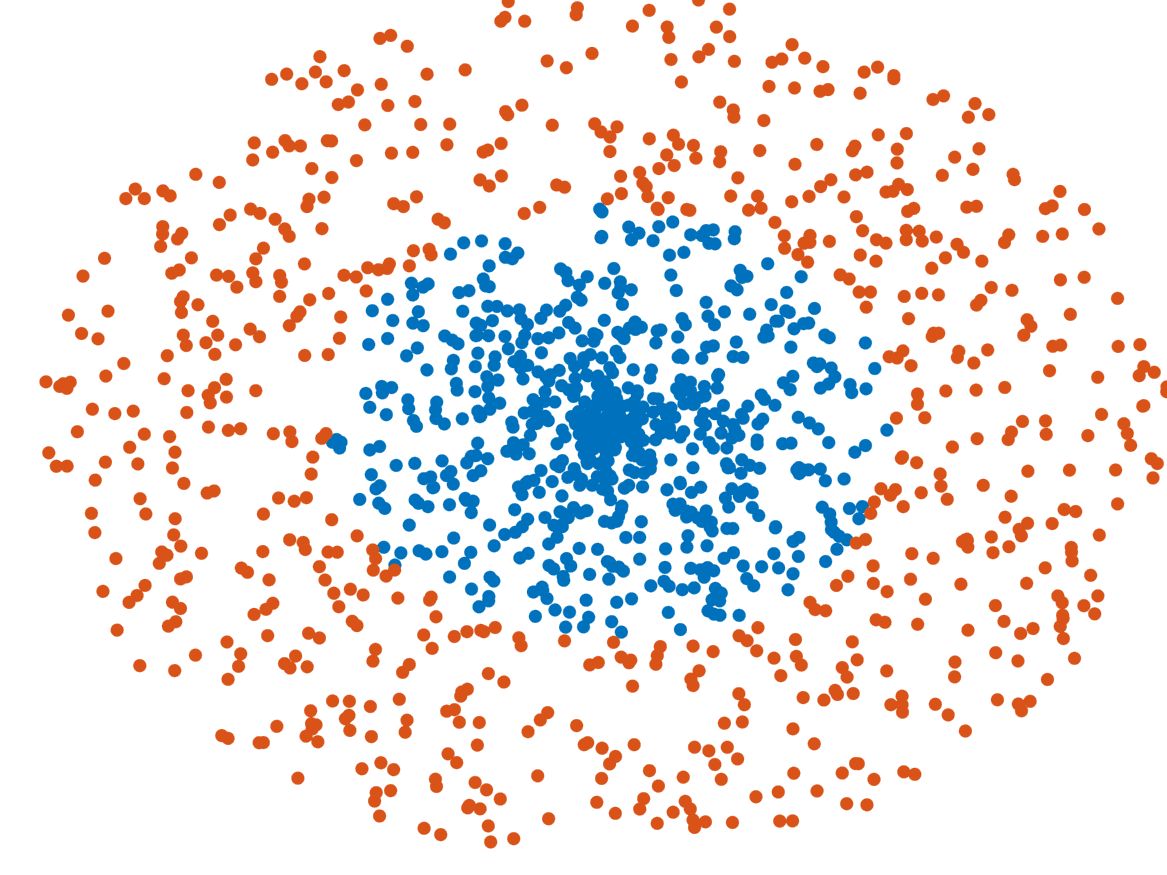
\includegraphics[width=45mm]{Circle-train} & 
		\invisible<beamer|1>{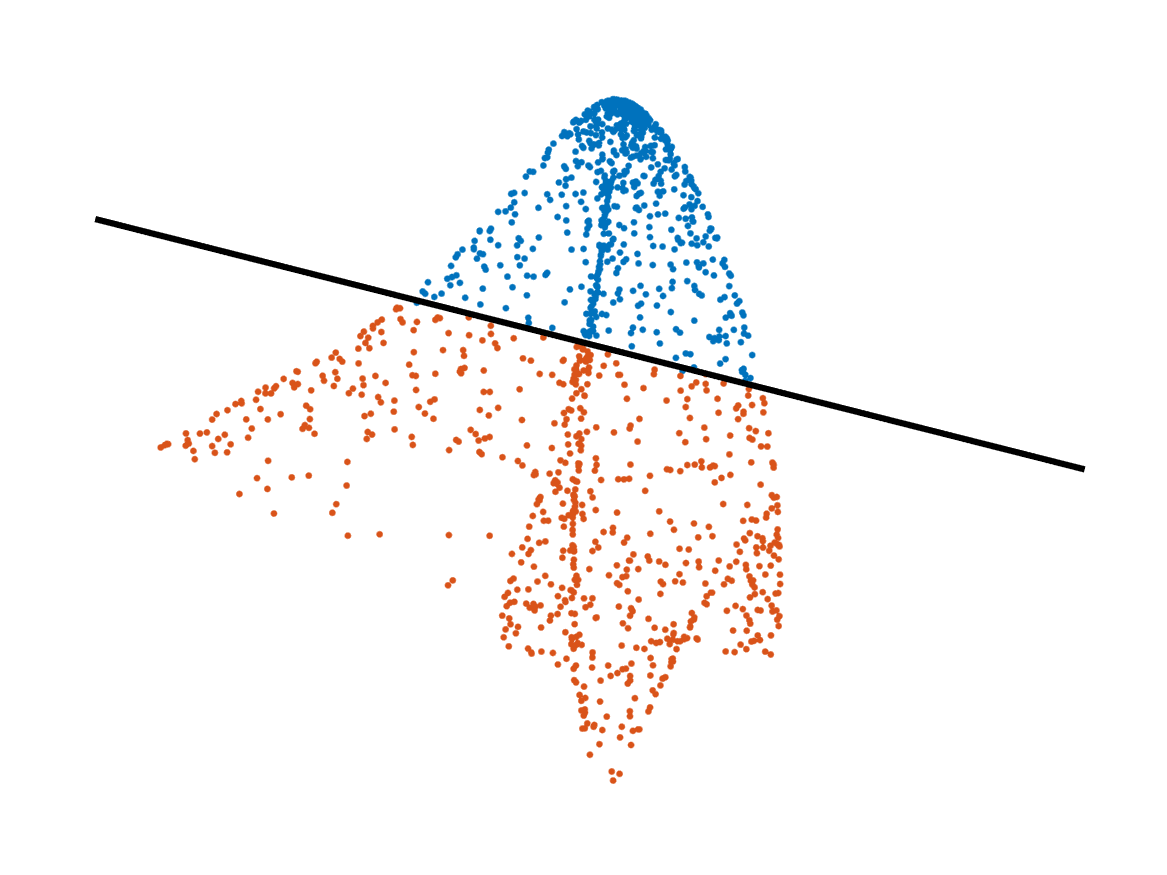
\includegraphics[width=45mm]{Circle-proptrain} }\\
		input features & \invisible<beamer|1>{transformed features}
	\end{tabular}
\end{center}

\bigskip

\invisible<beamer|1>{{\bf Goal/Trick}

Embed the points in higher dimension and/or move the points to make them
linearly separable}

\only<beamer|2>{}
\end{frame}